\documentclass[utf8x]{ctexart}
% \documentstyle[...,spconf,...]{article}
\usepackage{spconf,amsmath,graphicx}
\usepackage{hyperref}
\usepackage{array, caption, tabularx,  ragged2e,  booktabs}
\usepackage[round]{natbib}
\usepackage[T1]{fontenc}
\usepackage{lmodern}
\usepackage{dsfont}

% Example definitions.
% --------------------
\def\x{{\mathbf x}}
\def\L{{\cal L}}

% Title.
% ------
\title{EE5183 FinTech Final Project Report}
%
% Single address.
% ---------------
\name{Tadeo Hepperle, Student ID: A11922105\thanks{Thanks to AviviD Innovative Media.}}
\address{NTU National Taiwan University, Lecturer: Che Lin (林澤) }
%
% For example:
% ------------
%\address{School\\
%	Department\\
%	Address}
%
% Two addresses (uncomment and modify for two-address case).
% ----------------------------------------------------------
%\twoauthors
%  {A. Author-one, B. Author-two\sthanks{Thanks to XYZ agency for funding.}}
%	{School A-B\\
%	Department A-B\\
%	Address A-B}
%  {C. Author-three, D. Author-four\sthanks{The fourth author performed the work
%	while at ...}}
%	{School C-D\\
%	Department C-D\\
%	Address C-D}
%
\begin{document}
%\ninept
%
\maketitle
%
\begin{abstract}
  Amazon reviews are important for purchase decisions and their integrity is essential to the online platforms reputation. That is why immoral businesses have an incentive to publish fake reviews. In this paper we explore different machine learning models to detect fake reviews based on a combination of textual and numerical features. Our models use pretrained BERT embeddings as a base and achieve AUROC and AUPRC scores of up to 0.933 and 0.970 respectively.
  As a main innovation we allow our models to take a look at contextual reviews for the same Amazon product to better understand if a review is fake or not.

\end{abstract}
%
\begin{keywords}
  BERT, NLP, fraud detection, neural networks, sentiment analysis
\end{keywords}
%
\section{Introduction}
\label{sec:intro}

We take a look at a dataset consisting of Amazon reviews that were either real or fake. Real meaning "genuine" and fake meaning "likely forged".
Because the majority of online shop customers rely on reviews when making their purchase decisions it is important for a platform like Amazon to ensure the reviews reflect the real qualities of a product and are not misused as a marketing instrument by unethical businesses.
To detect fake reviews we propose two different neural network models that both make heavy use of a BERT architecture to generate text embeddings that are useful in the binary classification. To see how our best model performs in action you can check out \href{https://tadeohepperle.com/amazon-fake-reviews/}{this little online game}, where you can compete against our model yourself in real-time.

\subsection{Group Members}

We were 5 people in our group: Jenny and Tim took part in researching sources, background information and cleaning the data. They also made a big part of the presentation. Zow, Miguel and me came up with the 3-BERT model and trained all models on GPU-accelerated machines. I (Tadeo) coded the web-demo and the Context Embedding Model.

\subsection{Previous Work}

Previous work on fake review detection was done by other researchers however most focussed on either the use of textual or non-textual features. For example \cite{gu-budhkar} used transformer based models in a way that they transformed all features into text, reducing the problem domain to a mere binary text classification. \cite{mohawesh2021fake} used transformers combined in ensemble methods to classify texts. They also take the context of a review into consideration. \cite{weng2022detection} also detected Chinese fake reviews using pretrained language models. Combining these approaches is one of the aims of our project.

\section{Material and Methods}
\label{sec:format}


\subsection{Data and Preprocessing}

We used a dataset uploaded by Github user aayush210789 for our report, published \href{https://github.com/aayush210789/Deception-Detection-on-Amazon-reviews-dataset}{here on Github}. The data is from a corpus of reviews published by Amazon and was internally labeled as fake or real.
The dataset consists of a CSV file with columns shown in table~\ref{tab:feat1}.
\begin{table}[ht]
  \centering
  \caption{Original features}
  \label{tab:feat1}
  \begin{tabular}{l p{6cm}}
    Feature        & Description                                                                                      \\
    \hline
    review\_title  & title of the review                                                                              \\

    review\_text   & content/text of the review, mostly moderately long text                                          \\

    rating         & 1-5 star rating for the product                                                                  \\

    verified       & 1 if there was a verified purchase before the review was submitted, else 0                       \\

    label          & 0 for a real review, 1 for a fake review                                                         \\
    product\_id    & every Amazon product has a unique alphanumerical id                                              \\
    product\_title & title of the product                                                                             \\
    category       & the category of the product, in total 30 categories were present, such as PC, Baby, Books, \dots \\
  \end{tabular}
\end{table}

There are 10,500 fake and real reviews each, such that imbalance was not an issue.
The reviews encompassed 18857 Amazon products with unique IDs.

As Fig~\ref{fig:verified} shows, fake reviews tend to be less frequently verified purchases than real reviews. In contrast, there is no relationship between fake reviews and rating, see Fig~\ref{fig:rating}.

\begin{figure}[htb]
  \centering
  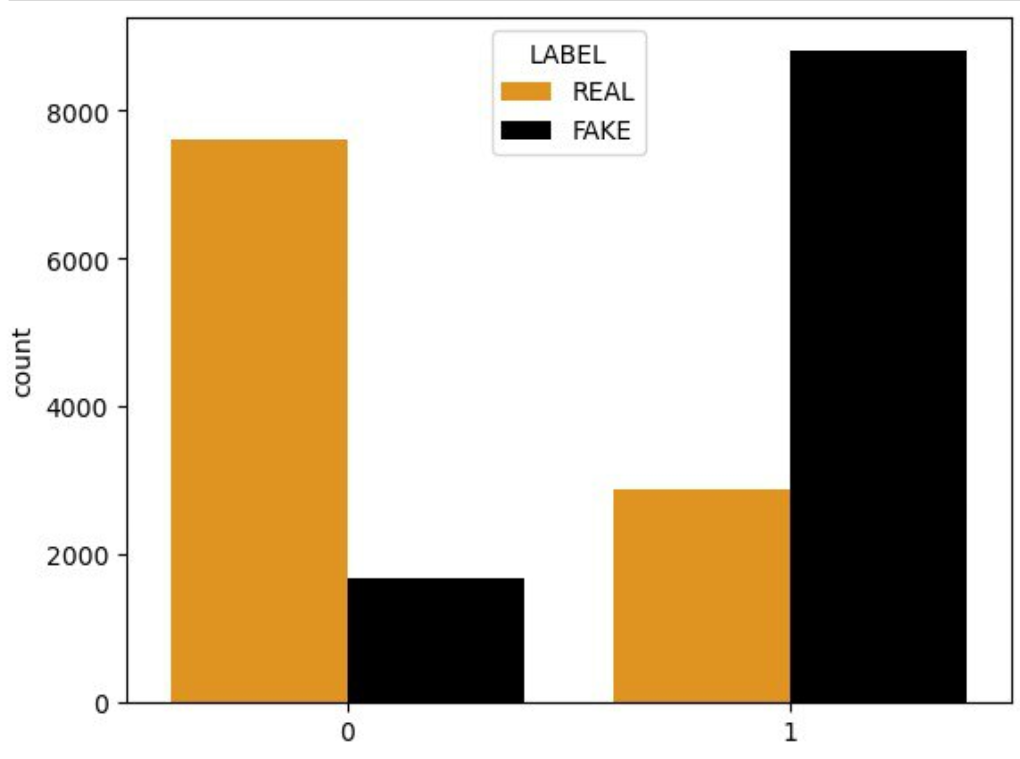
\includegraphics[width=0.48\linewidth]{./verified.png}
  \caption{Verified purchases}
  \label{fig:verified}
\end{figure}

\begin{figure}[htb]
  \centering
  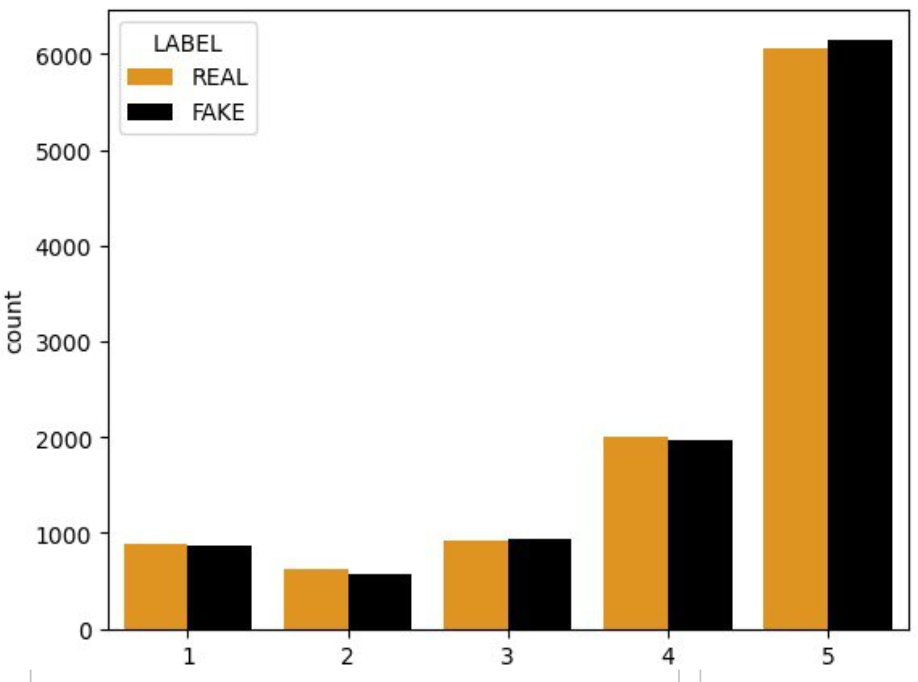
\includegraphics[width=0.48\linewidth]{./rating.png}
  \caption{Ratings}
  \label{fig:rating}
\end{figure}

\subsubsection{Scraping additional Data}

We discovered that most products were still listed on Amazon under the same product\_id and wrote a script that made 18857 requests to the corresponding Amazon websites, that are available under "www.amazon.com/dp/product\_id". For more than 86\% of the products (16,309 items) we were able to save the HTML content. This was 26.4 GB of data. For each of the products extracted from the HTML the features from table~\ref{tab:feat2}.

\begin{table}[ht]
  \centering
  \caption{Scraped features}
  \label{tab:feat2}
  \begin{tabular}{l p{6cm}}
    Feature       & Description                                                                                            \\
    \hline
    rating\_count & how many ratings a product had in total                                                                \\
    rating\_avg   & the average rating on a continuous scale from 1.0 to 5.0                                               \\
    rating1       & percentage of ratings that were 1 star                                                                 \\
    rating\dots   & percentage of ratings that were \dots stars                                                            \\
    rating5       & percentage of ratings that were 5 stars                                                                \\
    reviews       & array of reviews on the front page of the product, with features displayed in table~\ref{tab:feat2rev}
  \end{tabular}
\end{table}

\begin{table}[ht]
  \centering
  \caption{Features of each Scraped Review}
  \label{tab:feat2rev}
  \begin{tabular}{l p{6cm}}
    Feature       & Description                                                                \\
    \hline
    review\_title & title of the review                                                        \\
    review\_text  & content/text of the review, mostly moderately long text                    \\
    rating        & 1-5 star rating for the product                                            \\
    verified      & 1 if there was a verified purchase before the review was submitted, else 0 \\
    helpfulness   & how many people found this review helpful                                  \\
  \end{tabular}
\end{table}

In total, we scraped 99,995 additional reviews from product front pages. These reviews can be helpful because they give context: If a review is overly positive it might be fake, but if the most helpful reviews for this product are also all very positive it might be more likely to be genuine.

Using only products, for which we were able to scrape additional data, 18,107 labeled reviews remained.
There was a slight bias towards real reviews (52\% real vs 48\% fake).

\subsubsection{Splitting the Data}

The data was randomly split into 3 parts: 70\% of the reviews (12674) for the train set, 20\% (3641 reviews) for the validation set, 10\% (1792 reviews) for the test set.

\subsection{Methods}

We propose two different models: The 3-BERT model just uses the columns from the initial dataset. The Context Embedding Model tried to use the context information of the review (e.g. what do other reviews say about the product) to produce better predictions. In theory the Context Embedding Model should be more powerful, because it has access to a superset of the 3-BERT model data.

\subsubsection{3-BERT Model}

The 3-BERT model architecture can be seen in \ref{fig:3bert}. It uses a pretrained BERT model, that is fine-tuned to our task during training. This BERT model converts the review text, review title and product title into a 768 dimensional embedding each. This is done by taking the embedding of the [CLS] token, that is inserted before the text tokens itself, as the text embedding.
The 30 categories and 5 rating options were one-hot encoded and form together with the verified-flag a 36-dimensional vector. This is fed through a 6 layer deep fully connected neural network with dropout together with the BERT embedding of the product and review title. The result is joined with the review text embedding and again put through a fully connected neural network.

\subsubsection{Context Embedding Model}

The context embedding model uses all features available from the tables presented above. A central idea of this model is to create not only text embeddings but consistent embeddings for an entire review. This "review embedding network" is then used with the same weights on labeled and scraped reviews because they share the same features. Fig~\ref{fig:ren} shows this architecture: BERT is used to get 768-dimensional embeddings for the review title and review text each. The sentiment analysis library "textblob" is used to form features "valence" and "subjectivity" for both title and text. Then all vectors are concatenated with "rating" and "verified". This big vector is then fed through an MLP layer to form the review's embedding. The review embedding network shares weights in all instances that it occurs in. We use a transformer encoder layer to feed the "review embedding" of each scraped review to get a joined representation. This gives us a context embedding, that is concatenated with all other product features to get a product embedding, see Fig~\ref{fig:cem}. This is then joined with the original review embedding for the product and put through a binary classification MLP to predict the final label.

\section{Results}
\label{sec:results}

Our models were trained with the Adam optimizer with binary cross entropy loss and used the huggingface model "distilbert-base-uncased" as a base.
The 3-BERT model used a learning rate of 0.000023 and 32 epochs with a batch size of 4. The total training time was 16.8 hours.
The context embedding model (CEM) had a learning rate of 0.001 and trained for 10 EPOCHS with a batch size of 256 which took 7 hours. Performance differences could be due to different training times, but our computing resources were sadly limited. We compared the models to a few simpler models we trained: Unimodal: a model that transforms all features to text features and use only one BERT for the predictions. MLP + BERT:  uses MLP on categorical data and BERT for text. BERT + NN: Fine-tuned BERT (reviews only) + simple 5 layer neural network on categorical features.
Table \ref{tab:results} shows the performance of all models in terms of AUROC and AUPRC values on unseen test data.

\begin{table}[ht]
  \centering
  \caption{Features of each Scraped Review}
  \label{tab:results}
  \begin{tabular}{r|cc}
    Model      & AUROC & AUPRC \\
    \hline
    Unimodal   & 0.620 & 0.610 \\
    MLP + BERT & 0.812 & 0.820 \\
    BERT + NN  & 0.839 & 0.819 \\
    3-BERT     & 0.933 & 0.925 \\
    CEM        & 0.731 & 0.970 \\
  \end{tabular}
\end{table}

Figure \ref{fig:3bertroc} and \ref{fig:3bertprc} show the ROC and PRC curves for the final 3-BERT model. This seems to be our best model, it also had the longest training time. In comparison, the vastly more complicated CEM surpasses it in terms of AUPRC but fails to provide a high quality ROC curve. Figure \ref{fig:cemroc} and \ref{fig:cemprc} show the curves for that model.

\begin{figure}[htb]
  \centering
  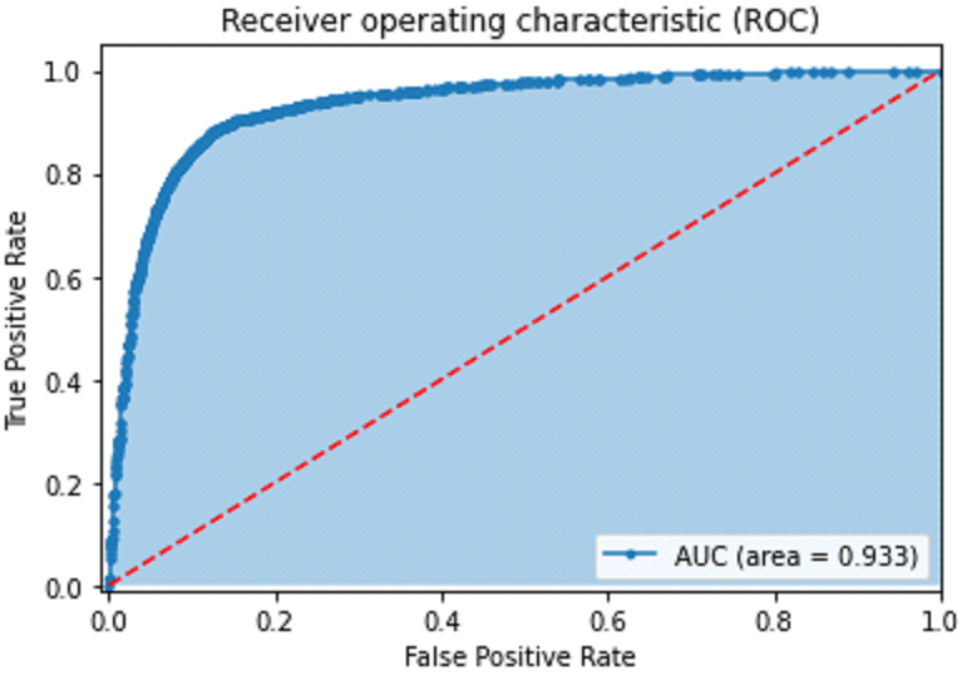
\includegraphics[width=\linewidth]{./3bertroc.png}
  \caption{3-BERT ROC}
  \label{fig:3bertroc}
\end{figure}

\begin{figure}[htb]
  \centering
  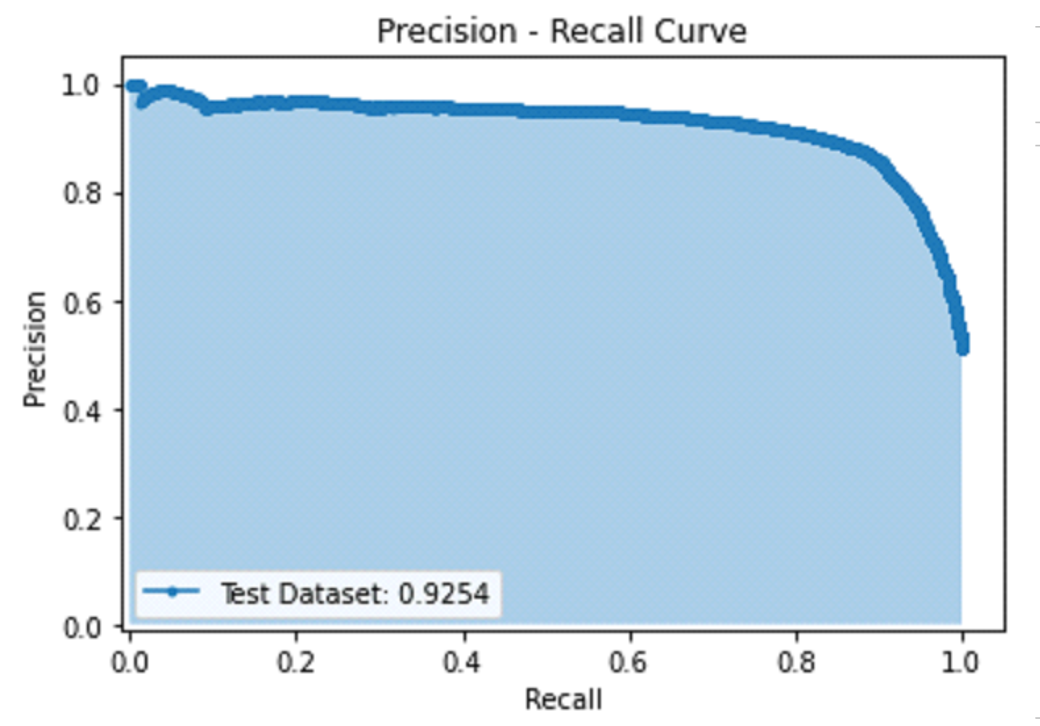
\includegraphics[width=\linewidth]{./3bertprc.png}
  \caption{3-BERT PRC}
  \label{fig:3bertprc}
\end{figure}

\begin{figure}[htb]
  \centering
  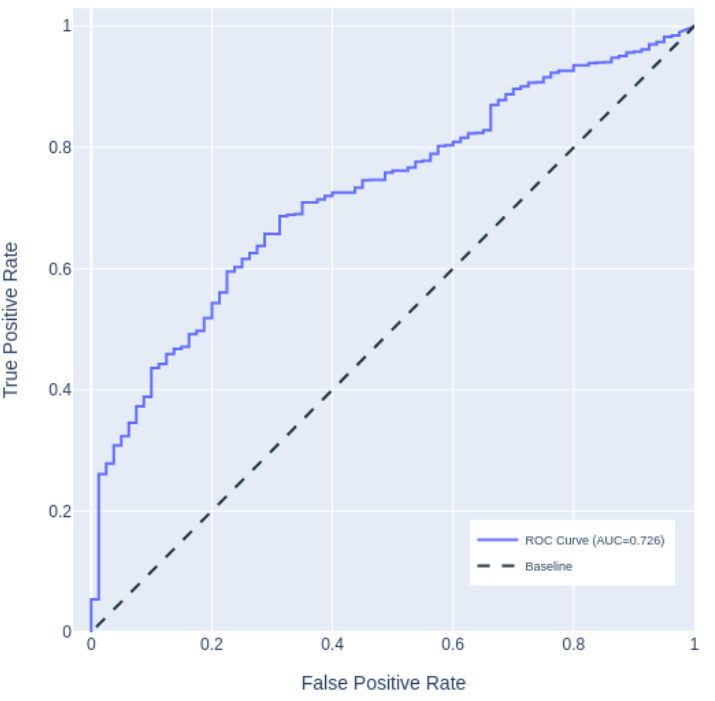
\includegraphics[width=\linewidth]{./cemroc.png}
  \caption{Context Embedding Model ROC}
  \label{fig:cemroc}
\end{figure}

\begin{figure}[htb]
  \centering
  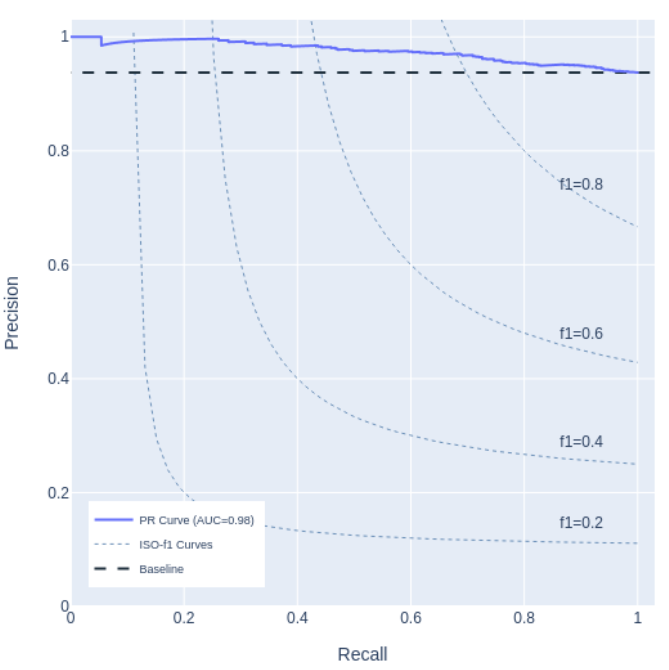
\includegraphics[width=\linewidth]{./cemprc.png}
  \caption{Context Embedding Model PRC}
  \label{fig:cemprc}
\end{figure}


\section{Discussion}

We were surprised that the 3-BERT model surpassed the Context Embedding model in terms of AUROC, because it uses less information. It could be the case that the transformer encoder layer in the Context Embedding Model simply adds too much complexity and makes it hard to learn the dependencies in the data. In the future it would be interesting to see what happens if we have more data available or different labels. We also feel like the models cannot be 100\% accurate in all cases, as they are a result of a different model used by Amazon.

\vfill\pagebreak

\section{REFERENCES}
\label{sec:refs}

% References should be produced using the bibtex program from suitable
% BiBTeX files (here: strings, refs, manuals). The IEEEbib.bst bibliography
% style file from IEEE produces unsorted bibliography list.
% -------------------------------------------------------------------------
% \bibliographystyle{IEEEbib}
% \bibliography{references}

\renewcommand\refname{Bibliography}
\bibliographystyle{plainnat}
\bibliography{references}


\pagebreak
\section{APPENDIX}



\begin{figure}[htb]
  \centering
  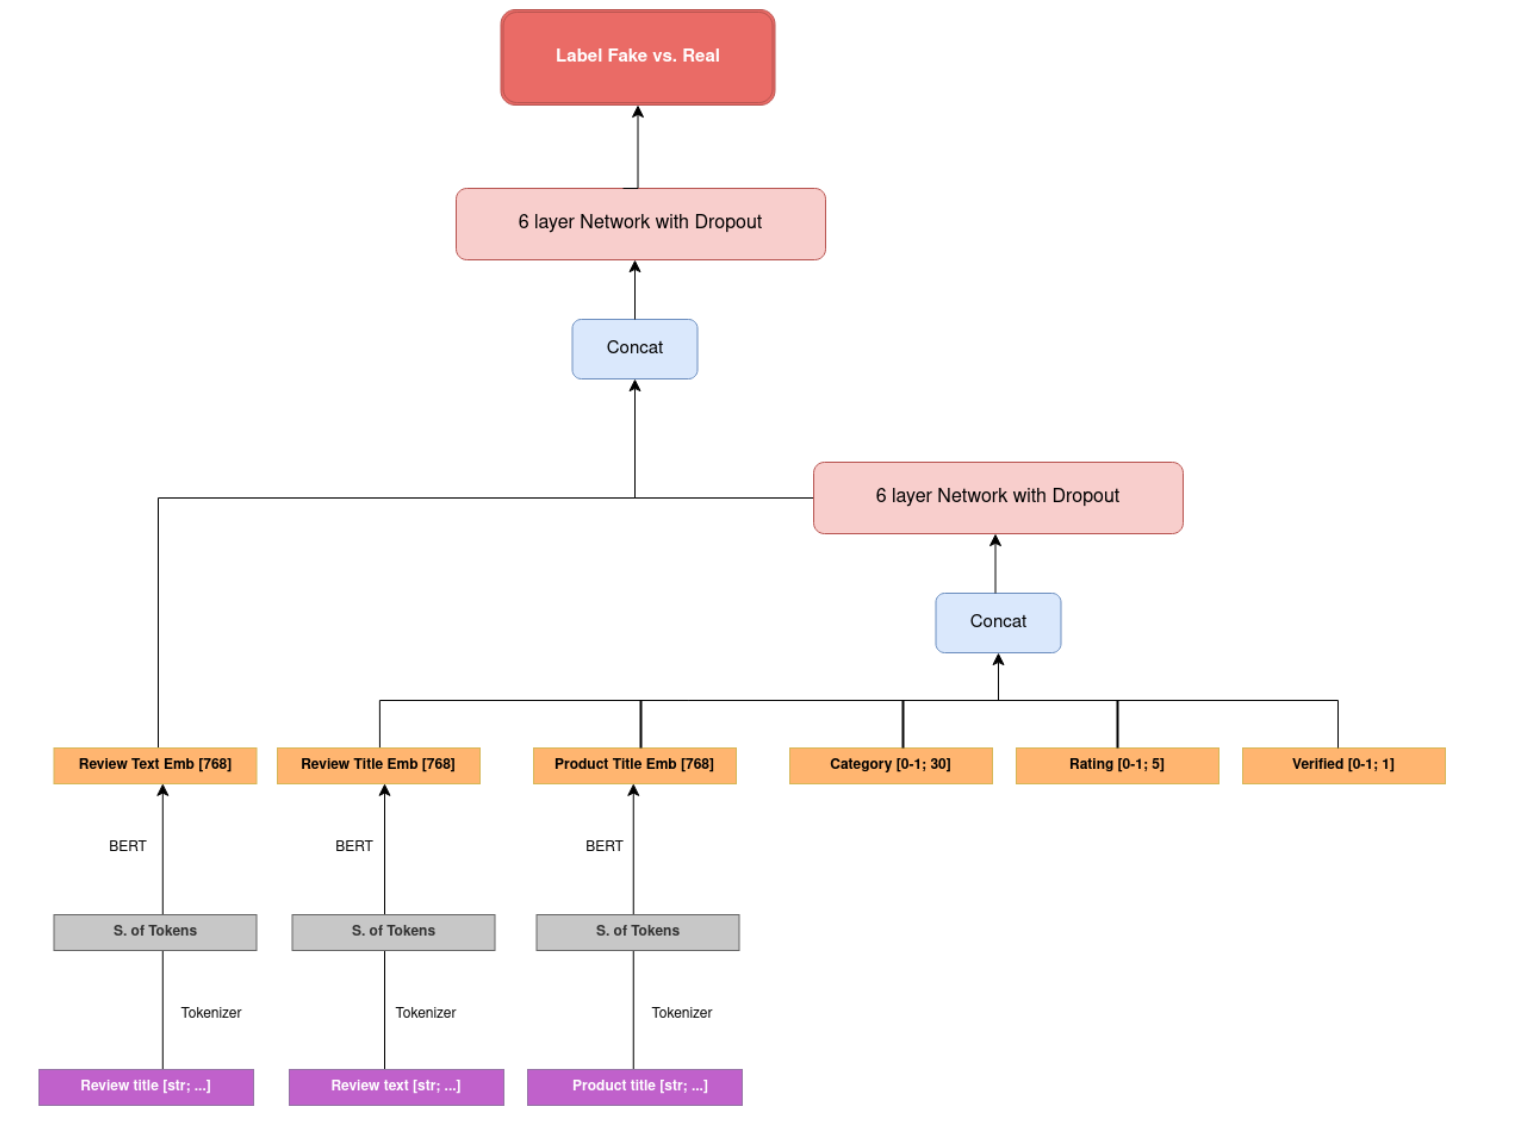
\includegraphics[width=\linewidth]{./3bert.png}
  \caption{Review Embedding Network}
  \label{fig:3bert}
\end{figure}

\begin{figure}[htb]
  \centering
  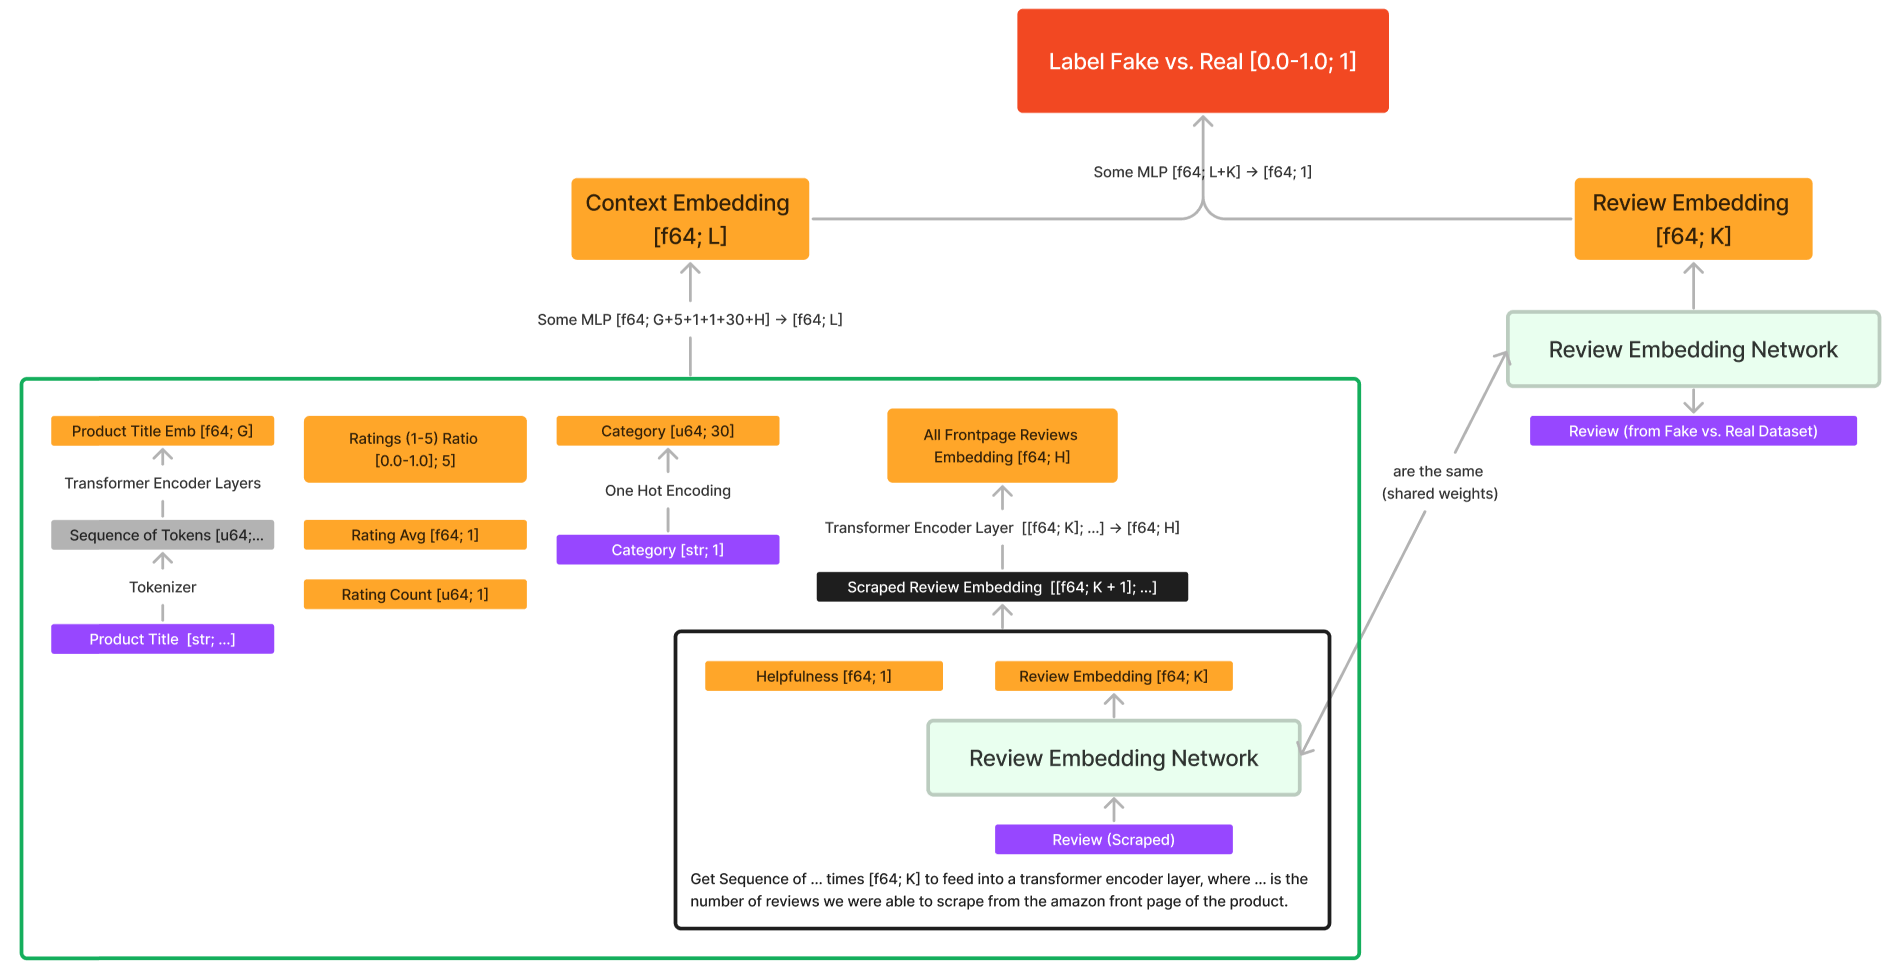
\includegraphics[width=\linewidth]{./cem.png}
  \caption{Context Embedding Model}
  \label{fig:cem}
\end{figure}

\begin{figure}[htb]
  \centering
  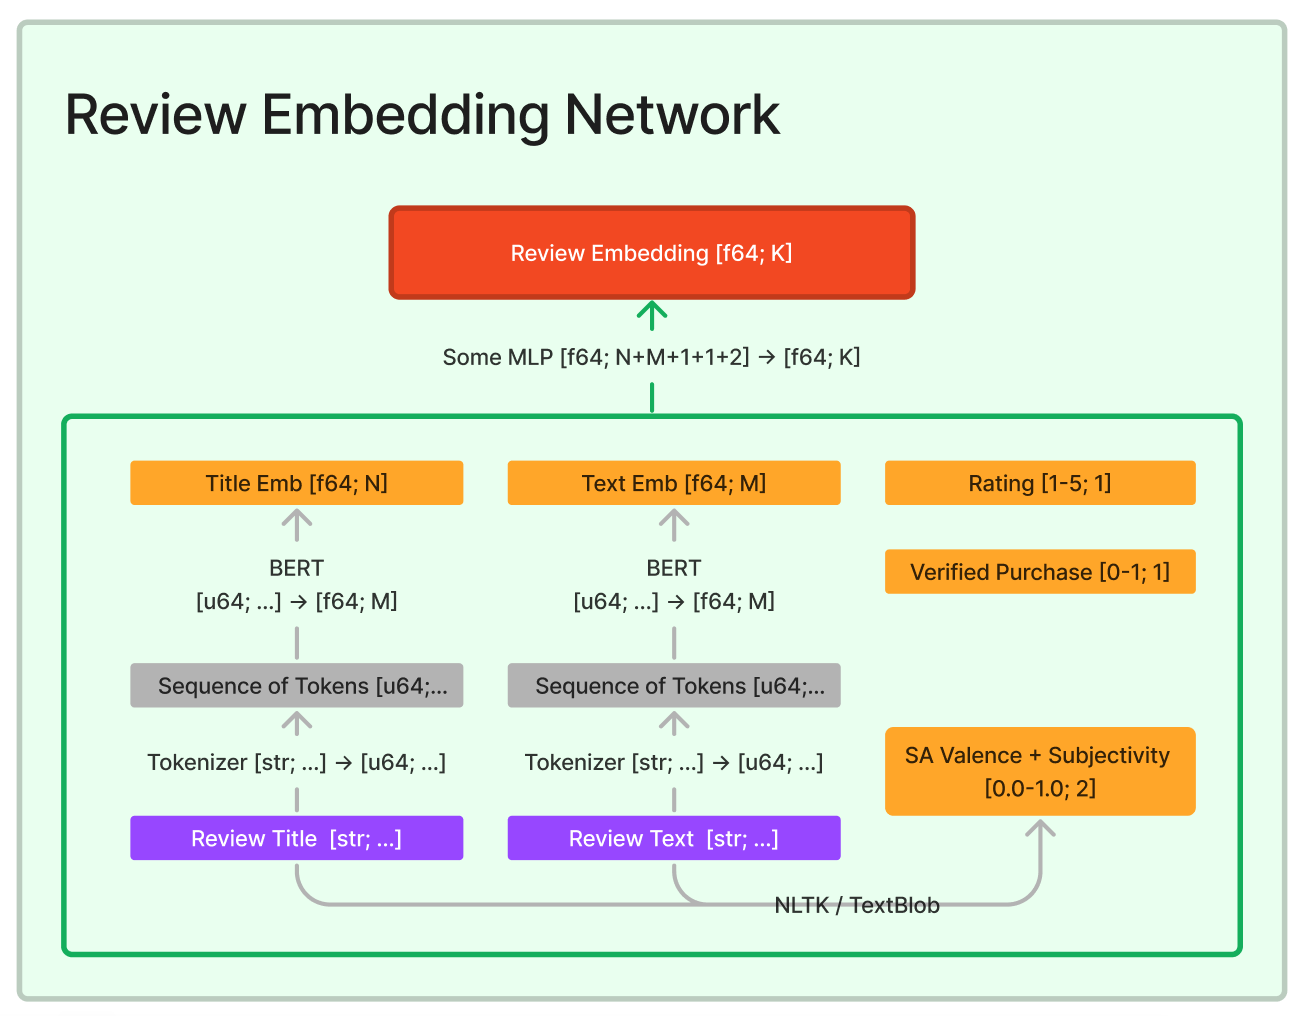
\includegraphics[width=\linewidth]{./ren.png}
  \caption{Review Embedding Network}
  \label{fig:ren}
\end{figure}




\end{document}
